\begin{figure*}[!t]
  \centering
  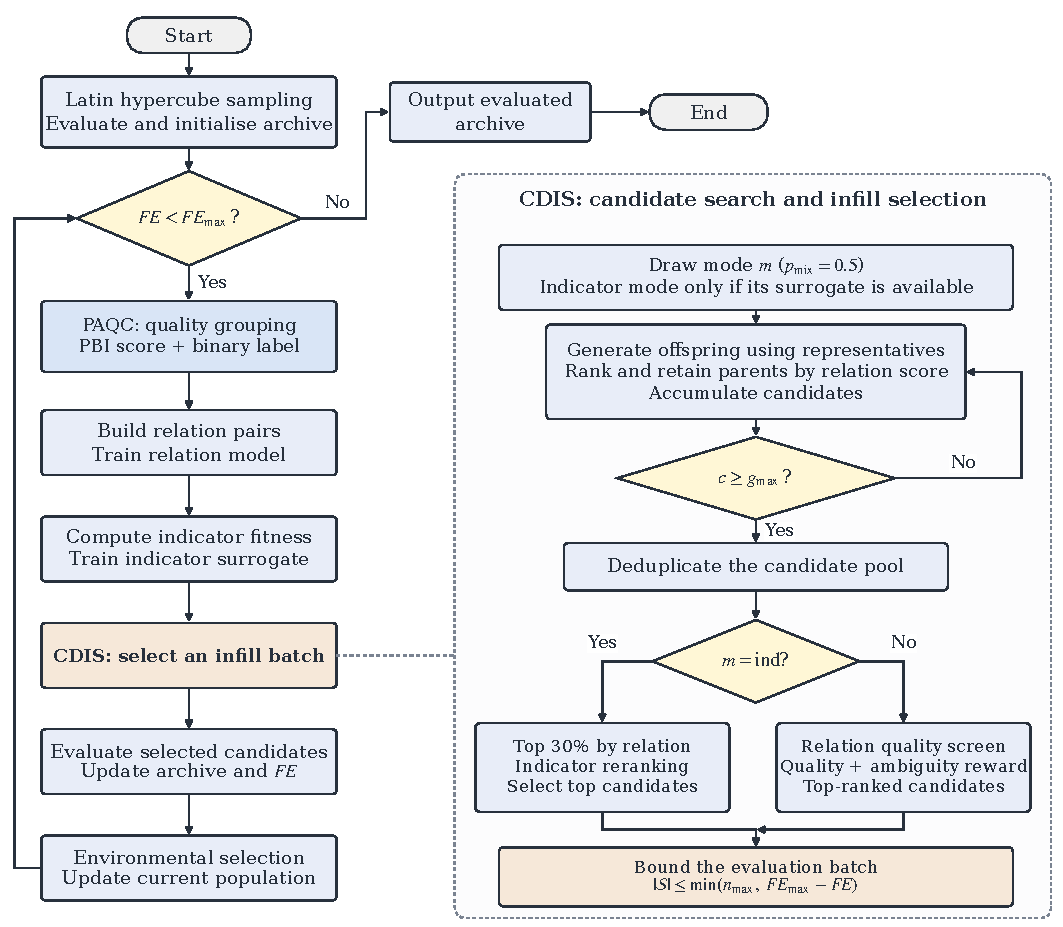
\includegraphics[width=0.98\textwidth]{figures/fig_framework.pdf}
  \caption{Flowchart of PACDIS. Left: the expensive-evaluation loop, with PAQC
  constructing the training groups and CDIS selecting the infill batch.
  Right: expansion of CDIS (dotted connector). A mode is drawn before the
  relation-guided search; $c$ counts the generated candidates and $g_{\max}$
  bounds their accumulation. Indicator mode is drawn with probability
  $p_{\mathrm{mix}}=0.5$ when its surrogate is available; otherwise exploration
  mode is used. The selected mode determines the final selection criterion:
  indicator mode applies quantile screening with retained-set completion, and
  exploration mode ranks the whole pool by \eqref{eq:expscore} under the single
  parameter $\beta$. In both cases the batch is bounded by $n_{\max}$ and by the
  remaining evaluation budget. Detailed safeguards are given in
  Algorithms~\ref{alg:framework} and~\ref{alg:cdis}.
  \label{fig:framework}}
\end{figure*}
